\documentclass{ledger}

%AUTHOR: This is a bare-bones template into which you may put your paper to aid in formatting your submission to Ledger. Note that to work properly, you must have the files "ledger.cls", "ledgerbib.bst", and the folder "images" on hand. 

%AUTHOR: the preferred method to generate PDF output is to use 'pdflatex'
%To clean up after a successful build, try: 'latexmk -c main.tex'

%EDITOR: in ledger.cls replace logoNewUC.png with logoNew.png prior to publication 


%EDITOR: replace X's to set the data for the header and footer
\newcommand{\thefirstpagenum}[0]{X}
\newcommand{\thelastpagenum}[0]{X}
\newcommand{\theyear}[0]{2024}
\newcommand{\thevol}[0]{X}
\newcommand{\thedoi}[0]{Asset Returns and Risk Projection}
\newcommand{\ledgerpages}[0]{\thefirstpagenum-\thelastpagenum}


\usepackage{paralist, caption}
\usepackage{booktabs} % For better table formatting
\usepackage{multirow} % For vertical centering across rows

\usepackage{tabularx}
\newcolumntype{Y}{>{\raggedleft\arraybackslash}X}
%\usepackage{siunitx} % For aligning numbers at the decimal point

%\usepackage[paperheight=16cm,paperwidth=12cm,textwidth=10cm]{geometry}

\usepackage{amssymb} %for the checkmarkts
\usepackage{rotating} % for sidewaystable

%AUTHOR: please set these to generate correct PDF metadata
\hypersetup{pdfauthor={iCapital Portfolio Analytics Research Group}, pdftitle={Asset Returns and Risk Projection: Technical Manual}}

%EDITOR: set the correct pageination during layout
%\setcounter{page}{\thefirstpagenum}


%AUTHOR: this can be used to highlight changed text, surround with \edit{} and
%uncomment either to determine color
%\newcommand{\edit}[1]{{\color{red} #1}}
\newcommand{\edit}[1]{#1}
	
\overfullrule=10pt

\title{Asset Returns Projection}

\author{iCapital Portfolio Analytics Quantitative Research Team}

%\author{Firstname A. Lastname,\thanks{BTC/BCH/ETH ADDRESS}\thanks{F. A. Lastname (f.lastname@abc.edu) is a fictional author and researcher at the Centre for Blockchain Technology at the University of Central Wakanda, Birnin Zana, Wakanda} Firstname Q. Lastname,\thanks{F. Q. Lastname (firstname.lastname@businessname.ca) is  Director of Network Science at the Blockchain Center of Canadia.}}

\pagestyle{pagemain}


%The Author should select the appropriate pretitle below:
\pretitle{
  %\centering \selectfont LEDGER \LaTeX \ TEMPLATE \par
  %\centering \selectfont REVIEW ARTICLE \par
  %\centering \selectfont RESEARCH ARTICLE \par 
  %The Author should not remove the following text:
  \centering \large Technical Manual for \par 
  \fontsize{24pt}{28pt}\selectfont} % Title is centered and at 24pt


\begin{document}

\maketitle

\thispagestyle{pagefirst}

%\begin{abstract}
%Lorem ipsum dolor sit amet, consectetur adipiscing elit, sed do eiusmod tempor incididunt ut labore et dolore magna aliqua. Venenatis cras sed felis eget velit aliquet sagittis. Dis parturient montes nascetur ridiculus mus mauris vitae. Bibendum at varius vel pharetra vel. Amet mattis vulputate enim nulla aliquet porttitor. Urna porttitor rhoncus dolor purus non enim praesent elementum. Velit aliquet sagittis id consectetur purus ut faucibus pulvinar. Quam adipiscing vitae proin sagittis nisl rhoncus mattis rhoncus urna.\cite{Nakamoto2008} Risus quis varius quam quisque id. Habitasse platea dictumst quisque sagittis purus sit amet volutpat consequat.

%AUTHOR: keywords are OK to show for Review article, will be hidden and added to metadata for publication
%\begin{keywords}
%\item Lorem ipsum.
%\item Dolor.
%\item Sit amet.
%\end{keywords}
%\end{abstract}

\section{Introduction and Scope}
This project involves inputting historical asset class data to get return and risk projections for individual assets on Architect. We use Principal Components Regression to accomplish this task. There are two main inputs to this project:
\begin{compactenum}
	\item The historical returns of asset classes;
	\item The risk and return estimates provided by external CMA providers. \\
\end{compactenum}

\begin{figure}[!ht]
\centering
	%\captionsetup{justification=centering}
	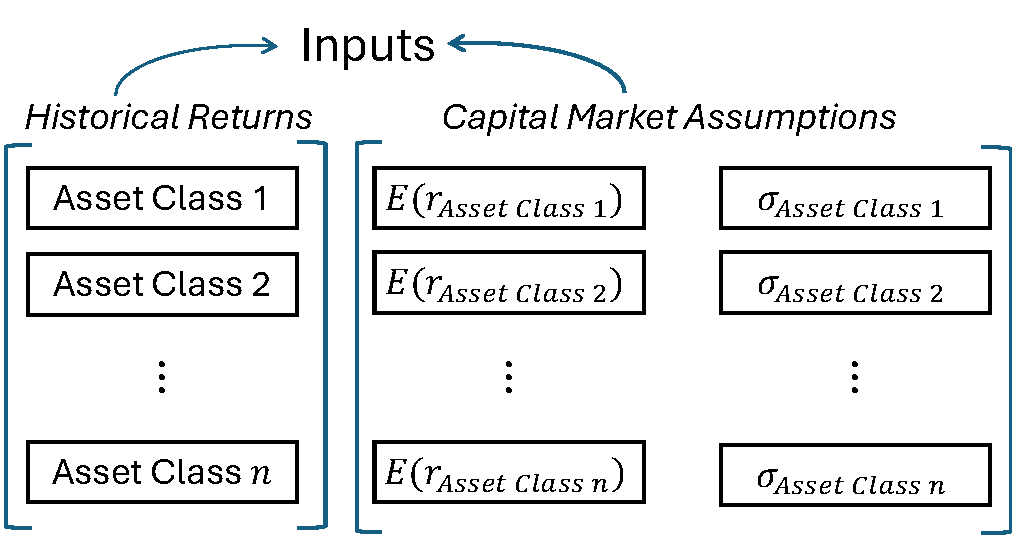
\includegraphics[width=250pt]{Inputs.pdf}
	 \caption{Inputs to the process.} ~\\
	%\label{graph1}
\end{figure}

The \textbf{outputs} to the process will be estimates of fund-level:
\begin{inparaenum}[$\bullet$]
	\item  future expected return;
	\item  and future expected risk
\end{inparaenum}
for each individual asset in Architect. We use \textbf{principal components regression (PCR)} to accomplish this task. 

\section{Methodology}
\begin{figure}[!ht]
\centering
	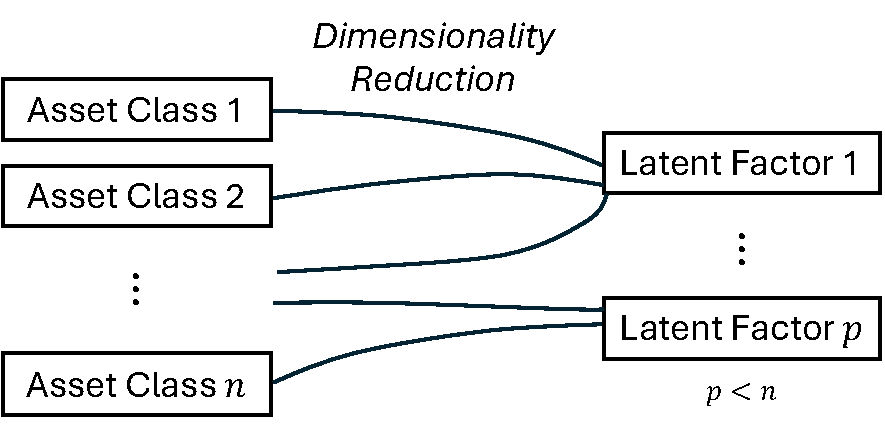
\includegraphics[width=400pt]{/Users/asheth/Library/CloudStorage/OneDrive-iCapitalNetwork/FactorPrediction/ProjectDescription/Step1.pdf}
	\caption{The first step in the methodology.} ~\\
\end{figure}

Principal components regression (PCR) is a technique used when the number of regressors is high, and are most likely correlated. Instead of regressing the dependent variable on all the explanatory variables, select principal components of the explanatory variables are used as regressors. One typically uses only a subset of all the principal components for regression; as a result, PCR could be interpreted as a kind of regularization procedure. It can also be viewed as a type of shrinkage estimator. \\

\begin{figure}[!ht]
\centering
	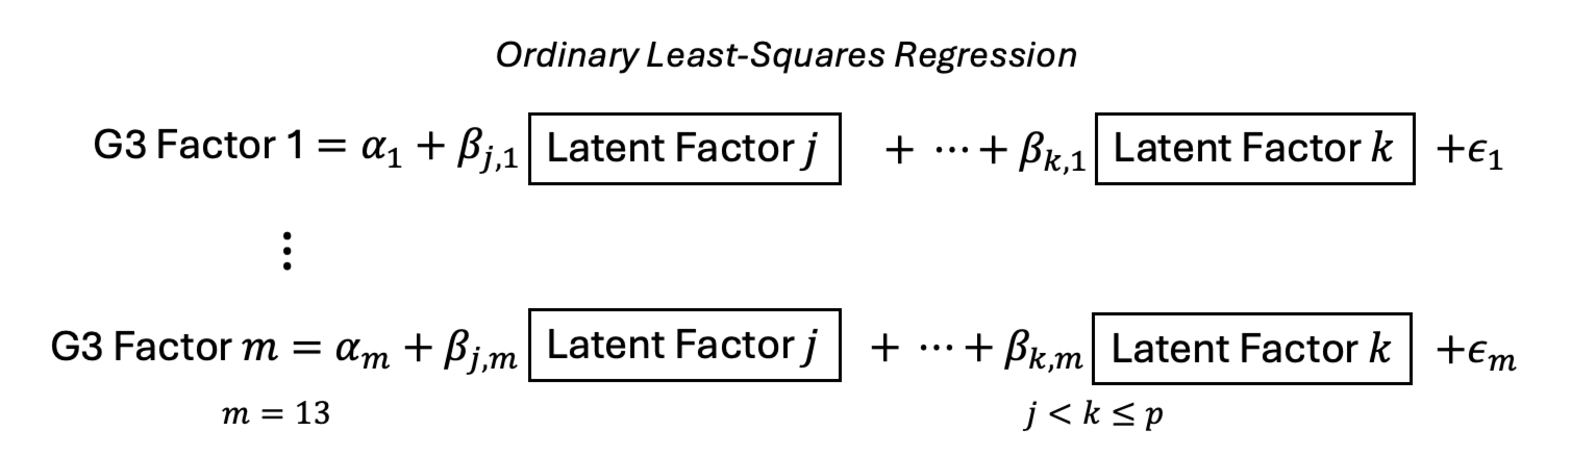
\includegraphics[width=375pt]{/Users/asheth/Library/CloudStorage/OneDrive-iCapitalNetwork/FactorPrediction/ProjectDescription/Step2.pdf}
	\caption{The second step in the methodology.} ~\\
\end{figure}

\subsection{Summary}

The basic methodology can be summed up in four steps. We do this for each of the 13 factors:
\begin{compactenum}
	\item Reduction of dimensionality of asset classes using principal components analysis, and selection of the optimal principal components using LARS Lasso. 
	\item Coefficient generation on reduced feature set via ordinary least-squares regression. Specifically, each G3 factor on the left-hand-side (LHS, dependent variable), and the optimal reduced feature set (the components from the LARS Lasso above) on the right-hand-side (RHS, independent variables). 
	\item Combine external CMAs with regression coefficients generated above to get future expected factor return and risk projections.  
	\item Use G3 factor loadings on future expected factor-projections to get asset-level projections. \\
\end{compactenum}

\begin{figure}[!ht]
\centering
	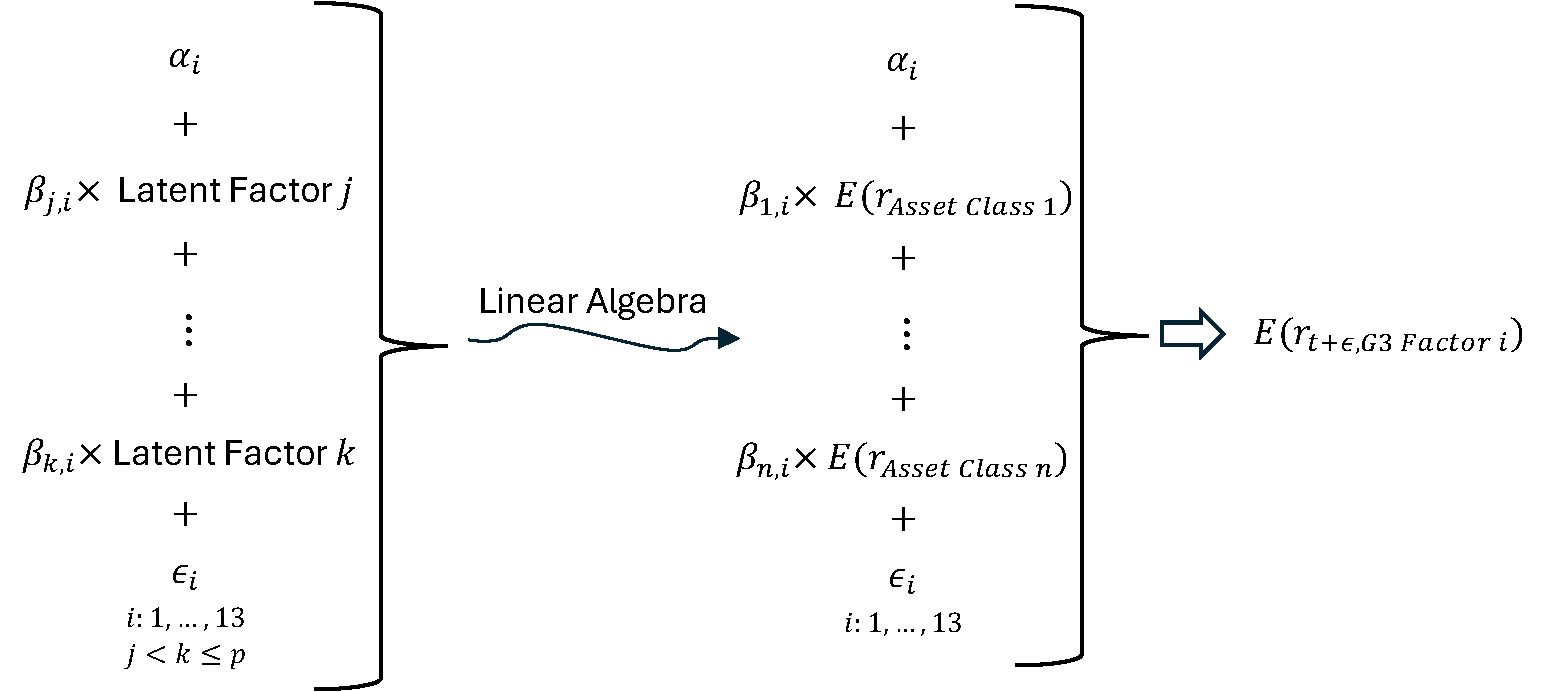
\includegraphics[width=425pt]{/Users/asheth/Library/CloudStorage/OneDrive-iCapitalNetwork/FactorPrediction/ProjectDescription/Step3.pdf}
	\caption{The third step in the methodology for a single factor. It is repeated for all factors.} ~\\
\end{figure}

\subsection{Potential Issues and Solutions}

Usually, the principal components which have a higher percent-variance-explained (the ones based on eigenvectors corresponding to the higher eigenvalues of the sample variance-covariance matrix of the explanatory variables) are selected as regressors. It should be noted, however, that for the purpose of predicting the outcome, the principal components with lower percent-variance-explained may also be important\footnote{When Kendall and Hotelling first proposed PCR in the 1950s, they proposed ``complete" PCR, which means replacing the original variables by \textit{all} the principal components. Which principal components are included in the final model is determined by looking at the explained variance of the parameter estimates. By the early 1980s, the term PCR had changed to mean ``incomplete PCR.''}. The logic behind this is simple -- PCR does not consider the response variables (our factors) when deciding which components to drop; that decision is based only on the magnitude of the percent-variance-explained within the components themselves.\\

%To resolve this, we use LARS Lasso to select the optimal number of components to keep. So the overall methodology can be described as follows:
%\begin{compactenum}
%	\item Perform a 10-fold cross-validation baseline ordinary least squares regression using all of the original independent variables (the original feature set). The mean of the cross-validation scores  from this regression is henceforth referred to as the  \textbf{\textit{baseline}} score. We use root mean square error (RMSE) for the cross-validation scores\footnote{Note that the number of folds, as well as the particular choice of score here is somewhat arbitrary. Other options were explored, and the results did not vary much.}.
%	\item Perform a cross-validated LARS Lasso regression on each of the principal components. Use the mean of the cross-validation RMSEs for each component to compare with baseline.
%	\begin{compactenum}[$\bullet$]	
%		\item The number of principal components that minimize the difference between their own mean cross-validation score and the baseline RMSE are the optimal number of components required for the regression. 
%	\end{compactenum}
%	\item For each dependent variable in the regression (our factors), we then use the optimal number of components for that respective component. Also, for each dependent variable, we store: the coefficients, the error terms, and the intercept.
%	\item We then use the Capital Market Assumptions to generate next-period return and risk measures for our factors, using the stored values above. \\
%\end{compactenum}

In this manner, we ensure that, both:
\begin{compactenum}[$\bullet$]	
	\item the maximum variance of the independent variables; \textit{and}
	\item the explanatory power of the independent variables \textit{on} the dependent variables, 
\end{compactenum}
are accounted for. \\

For details on $k$-fold Cross-Validation, and LARS Lasso, please refer to the Appendix.

\section{Results}

\subsection{Data}
%
The methodology in this paper was inspired by Haddad et al (2020)\footnote{Haddad, V., S. Kozak, S. Santosh. 2020. Factor Timing. \textit{The Review of Financial Studies}, 33(5):1980–2018.}.  \\

The asset classes used are:
\begin{inparaenum}[(i)]
    \item Buyout and growth
    \item Commodity
    \item Emerging markets equities
    \item Emerging markets fixed income
    \item Event driven
    \item Fund of funds
    \item Global macro
    \item Hedged equity
    \item Long/short credit
    \item MultiStratHF
    \item MultiStratPE
    \item Non-US developed equities
    \item Private debt
    \item Private real asset
    \item Real estate
    \item REITs
    \item Secondaries
    \item US equities
    \item US fixed income. 
\end{inparaenum} Note that the asset class data is \textit{desmoothed} (see below for details), and this ensures that all quarterly data is converted to monthly. \\

The factors used are:
\begin{inparaenum}[(i)]
    \item Alt commodities
    \item Alt HF crowding
    \item Alt oil
    \item Alt trend
    \item Emerging markets
    \item Equity market
    \item Equity momentum
    \item Equity quality
    \item Equity smallcap
    \item Equity value
    \item Fixed credit
    \item Fixed duration
    \item US dollar. \\
\end{inparaenum}

Correlations for all time series can be seen in Figure \ref{fig:correlations}. Many correlations are positive, suggesting broad market factors tend to drive returns across asset classes. However, not all are positive, and even among the positive ones, the strength of correlations varies considerably. Equities, for example, tend to be highly correlated with each other: Alt HF Crowding, Emerging Markets, Equity Market, Equity Momentum, and Equity Quality. This suggests equity market returns are often driven by common underlying factors. Buyout and Growth is also highly correlated with many series, suggesting the multi-asset nature of buyout funds. Fixed Income shows very low correlation with most other asset classes, as do Commodities and Emerging Markets Fixed Income. As a final note, it should be noted that the asset classes are correlated, so Principal Components Analysis on them is justified. \\

\begin{figure}[!ht]
	\centering
	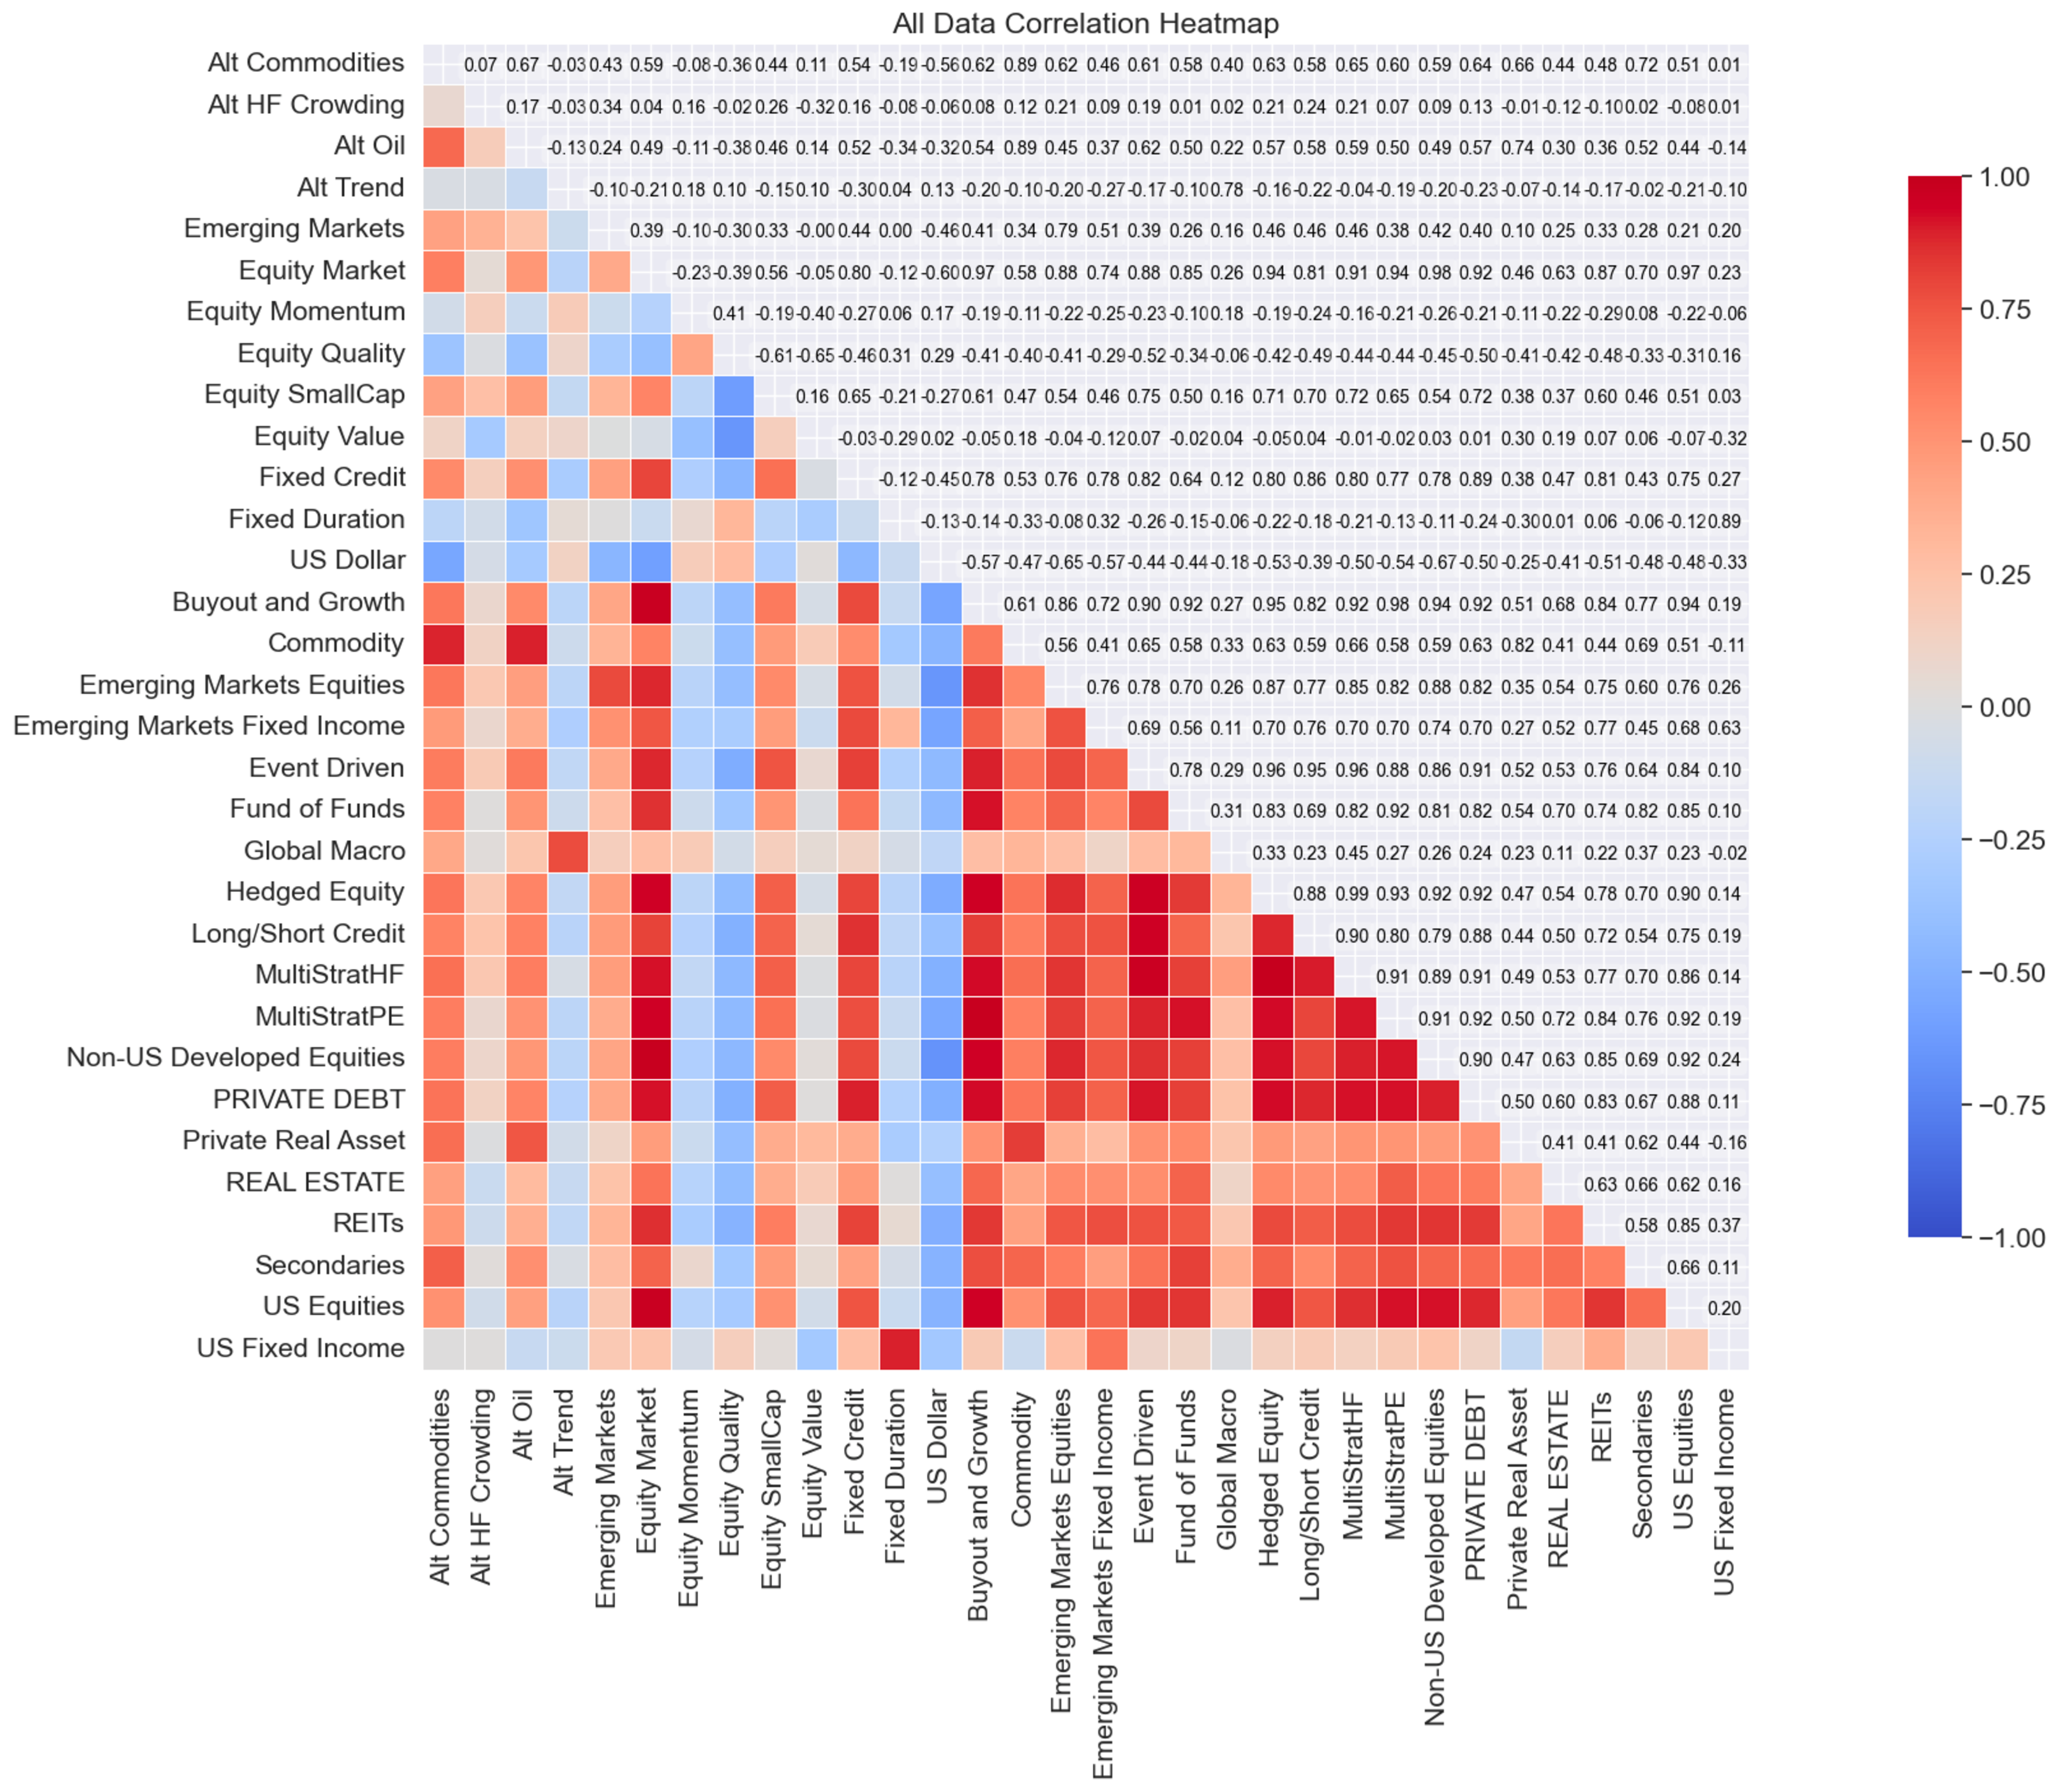
\includegraphics[width=430pt]{correlations.pdf}
	\parbox{430pt}{\caption{Correlations of all time series returns. \label{fig:correlations}}}
\end{figure}

The data is monthly and the months for which all series have data is October 31 2007 to July 31 2023. Also, we break up the dataset into training and testing in an 80\%-20\% split, respectively. To preserve the temporal sequence (and any potential serial correlation), we do not shuffle the data before splitting it into the train and test set. \\

Finally, we use the \textit{desmoothed} asset class returns, to ``convert'' the quarterly data into monthly data. For details on the desmoothing process, please refer to the Appendix. \\

Histograms for the standardized, desmoothed asset class returns can be seen in Figure \ref{fig:asset_class_histograms}. Some exhibit more positive skew (e.g. Global Macro, Real Estate) and others more negative skew (e.g. Event Driven). The dispersion also differs, with some sectors having tighter distributions (e.g. US Equities) compared to wider spreads in others (e.g. Long/Short Credit, Private Debt). REITs and Fund of Funds, are more concentrated around the mean. MultiStratHF and Secondaries, have a more even spread across the distribution. Hedged Equity has its peak slightly to the right of center, indicating a bias towards positive returns, while Commodity's peak is left of center, suggesting a bias towards negative returns.\\

\begin{figure}[!ht]
	\centering
	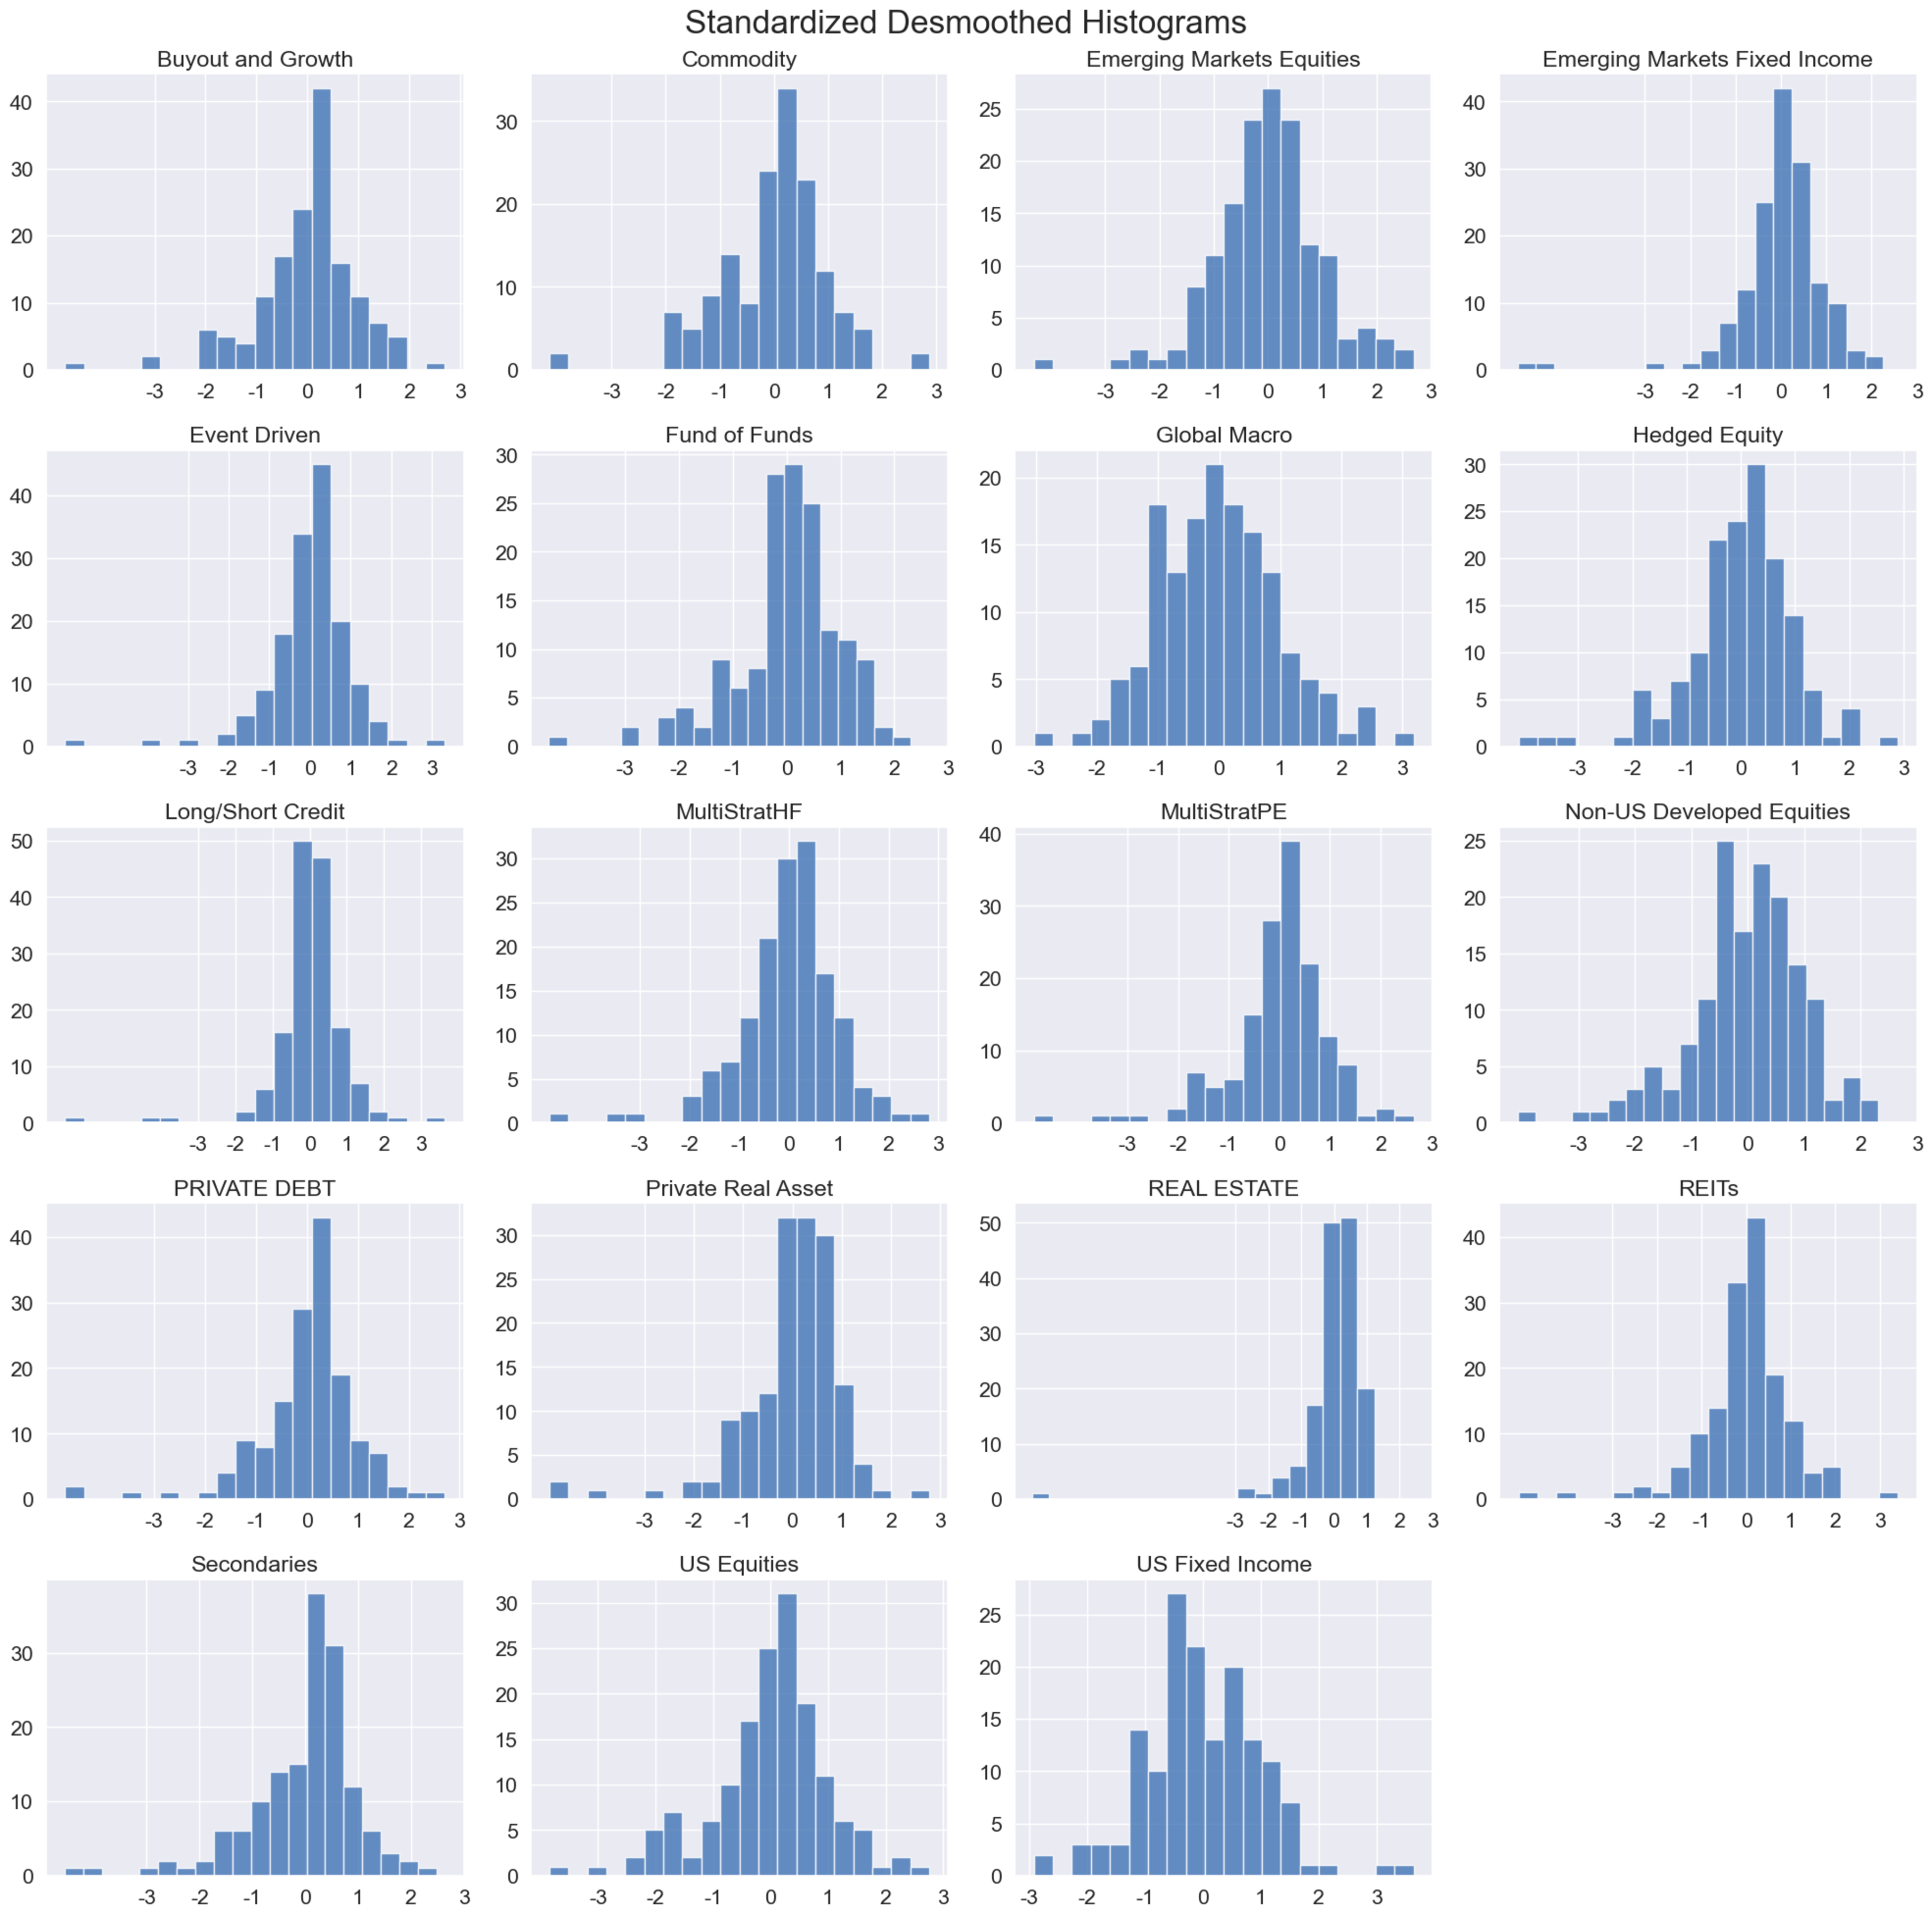
\includegraphics[width=430pt]{desmoothed_asset_class_histograms.pdf}
	\parbox{430pt}{\caption{Histograms of the standardized asset class returns. \label{fig:asset_class_histograms}}}
\end{figure}

\subsection{Generating a Baseline RMSE}

We run a 10-fold cross-validation on the training set of the original (unmodified) features, to get a baseline RMSE. We compare this with the RMSE on the test set. The results are shown in Table \ref{table:regression_rmse} below. \\

\begin{table}[ht]
\centering
\small % Adjust the font size 
\captionsetup{width=275pt, skip=4pt} % Adjust caption width and the space between the caption and the table
\caption{RMSE Results for OLS Regression for the Baseline. \label{table:regression_rmse}}
\begin{tabularx}{275pt}{>{\hsize=1.75\hsize}Y*{9}{>{\centering\arraybackslash\hsize=0.7\hsize}X}}
    \toprule
%    & \multicolumn{3}{c}{\textbf{OLS}} & \multicolumn{3}{c}{\textbook{Lasso}} & \multicolumn{3}{c}{\textbf{Ridge}} \\
%    \cmidrule(lr){2-4} \cmidrule(lr){5-7} \cmidrule(lr){8-10}
    \multirow{1}{*}{\textbf{Dependent Var}} & {\textbf{Train}} & {\textbf{Test}} & {\textbf{\%$\Delta$}} \\
    \midrule
	Alt Commodities & 0.0248 & 0.0213 & -14.21\% \\
	Alt HF Crowding & 0.0372 & 0.0468 & 25.83\% \\
	Alt Oil & 0.0539 & 0.0518 & -3.85\% \\
	Alt Trend & 0.0172 & 0.0154 & -10.03\% \\
	Emerging Markets & 0.0074 & 0.0093 & 26.38\% \\
	Equity Market & 0.0016 & 0.0039 & 142.51\% \\
	Equity Momentum & 0.0326 & 0.0826 & 153.02\% \\
	Equity Quality & 0.0220 & 0.0219 & -0.61\% \\
	Equity SmallCap & 0.0131 & 0.0193 & 47.20\% \\
	Equity Value & 0.0124 & 0.0242 & 95.38\% \\
	Fixed Credit & 0.0114 & 0.0141 & 22.87\% \\
	Fixed Duration & 0.0053 & 0.0095 & 80.60\% \\
	US Dollar & 0.0177 & 0.0146 & -17.96\% \\
    \bottomrule \\
\end{tabularx}
\end{table}

It should be stated, the absolute values of the RMS errors are small, and the results should be taken with a grain of salt. That said, there is considerable disparity between results. Equity Momentum, Equity Market, and Equity Value show significant improvement from the training set to the test set. These equity market factors have very similar drivers, and can be predicted easily using our unmodified asset classes. Fixed Duration shows considerable improvement as well. Alt Commodities, Alt Oil, and US Dollar exhibit negative percentage differences. This should not be surprising, as these factors are volatile. \\

\subsection{Principal Components Analysis}

We run a PCA on the training part of the RHS dataset. The results of the variance explained can be seen in Figure \ref{fig:variance_explained}. \\

\begin{figure}[!ht]
\centering
	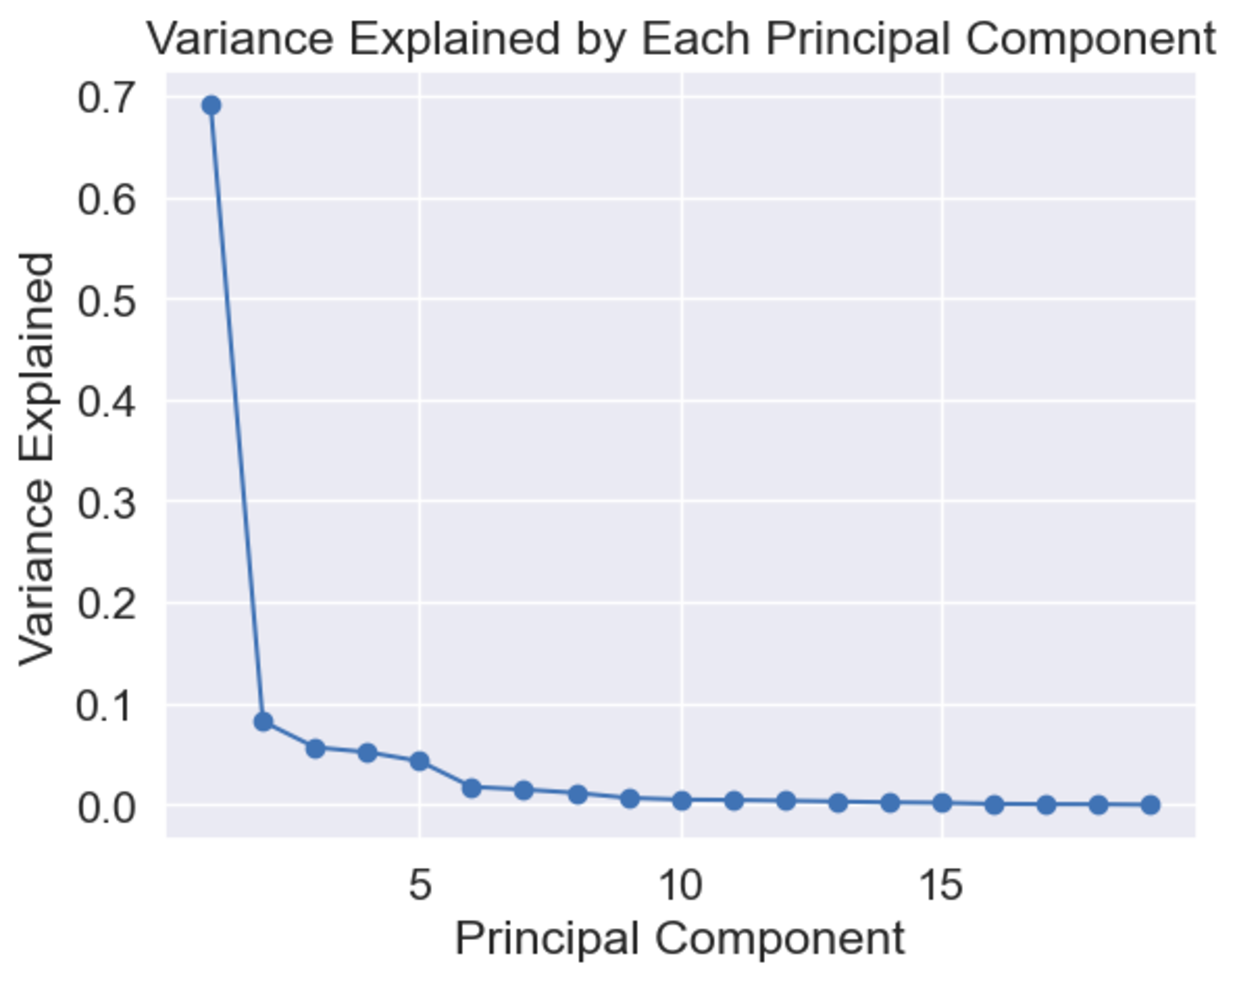
\includegraphics[width=300pt]{variance_explained.pdf}
	\caption{The variance explained by each principal component. The first component explains $\sim$69\% of the variance, with the rest of the components explaining 8\% or less, each. \label{fig:variance_explained}} ~\\
\end{figure}

\subsection{LARS Lasso}

The LARS Lasso helps us decide which principal components to keep, for each factor, since the percent-variance-explained metric only utilizes the asset class data, and not the factor data. In other words, there could be principal components with low percent-variance-explained, but they could be significant in explaining one of the factors. Table \ref{tab:pcs_kept} shows the principal components that are kept for each dependent variable. \\

\begin{table}[!ht]
\centering
\caption{Principal Components Kept for Each Dependent Variable. \label{tab:pcs_kept}}
\setlength{\tabcolsep}{3pt} % Reduces the space between columns
\footnotesize % Further reduces the text size
\begin{tabular}{r*{19}{>{\centering\arraybackslash}p{0.4cm}}c} % Defines narrower columns, and adds one for total PCs
	\toprule
		\multirow{2}{*}{\textbf{Factor}} & \multicolumn{19}{c}{\textbf{Principal Components}} & \multirow{2}{*}{\textbf{Total}} \\
	\cmidrule(lr){2-20}
			& \textbf{1} & \textbf{2} & \textbf{3} & \textbf{4} & \textbf{5} & \textbf{6} & \textbf{7} & \textbf{8} & \textbf{9} & \textbf{10} & \textbf{11} & \textbf{12} & \textbf{13} & \textbf{14} & \textbf{15} & \textbf{16} & \textbf{17} & \textbf{18} & \textbf{19} & \\
	\midrule
		Alt Commodities   & & x & x & x & x & & x & x & x & & & x & x & x & & x & x & & x & 13 \\
		Alt HF Crowding   & x & x & x & x & x & x & x & x & x & x & x & x & x & x & x & x & x & x & x & 19 \\
		Alt Oil           & x & x & x & x & x & x & x & & & x & x & x & x & x & x & x & x & x & & 16 \\
		Alt Trend         & & x & x & & & & x & & & & & & & & & & & x & & 4 \\
		Emerging Markets  & & x & x & x & & & & & x & & & x & & & x & x & & x & & 8 \\
		Equity Market     & x & x & x & & & x & x & x & x & & & x & x & & x & x & & x & & 12 \\
		Equity Momentum   & & & & & & & & & & & & & & & & x & & & & 1 \\
		Equity Quality    & & x & & & x & & x & & & & & x & & & x & x & & x & x & 8 \\
		Equity SmallCap   & & & x & x & x & x & x & x & x & & x & x & x & & x & x & & x & & 13 \\
		Equity Value      & x & & x & x & x & & & x & & & & x & x & x & x & x & & x & x & 12 \\
		Fixed Credit      & & x & x & & & & & & x & & & & & & & x & & & & 4 \\
		Fixed Duration    & & x & x & & x & & & & & & & x & & & & & & x & x & 6 \\
		US Dollar         & & x & x & x & & & & & x & & & x & & x & & & & x & x & 8 \\
	\midrule
		\textbf{Total} & 4 & 10 & 11 & 7 & 7 & 4 & 7 & 5 & 7 & 2 & 3 & 10 & 6 & 5 & 7 & 10 & 3 & 10 & 6 & \\
	\bottomrule \\
\end{tabular}
\end{table}

There is a significant variation in the number of principal components retained across different dependent variables. For instance, Alt HF Crowding retains all 19 components, suggesting that variance across these components is evenly spread, or the model relies heavily on capturing as much information as possible from the data. In contrast, Equity Momentum retains only one component, indicating that most of the useful variance can be captured by a single principal component. \\

The number of components retained can also suggest the complexity of the underlying patterns within each variable. A higher number of components might imply more complex interactions or more nuanced underlying structures. For example, Emerging Markets and US Dollar, retaining 7 and 8 components respectively, may indicate more complex financial behaviors or influences requiring multiple factors for adequate representation. \\

The total counts of each PC across all variables (shown in the last row) provide a useful overview of how often each PC is utilized. PCs with higher counts are more universally useful across multiple dependent variables, suggesting they capture more generalizable features of the data. PCs utilized less frequently may capture more specific, unique, or less significant aspects of the data. \\

\subsection{Principal Components Regression}

The results of the Principal Components Regression using the principal components selected from the LARS Lasso above are shown in Table \ref{table:scores_percent_differences_improvement}. Note that the ``Diff'' column shows the difference in the percent change of RMSE from the training to the test data, from OLS with the original features, to PCR with the reduced, transformed feature set. \\

\begin{table}[ht]
\centering
\small % Adjust the font size 
\captionsetup{width=425pt, skip=4pt} % Adjust caption width and the space between the caption and the table
\caption{Tain and Test Scores for Principal Components Regression, with Percent Differences for all Factors. OLS Results Included. \label{table:scores_percent_differences_improvement}}
\begin{tabularx}{425pt}{>{\hsize=1.5\hsize}Y*{5}{>{\centering\arraybackslash\hsize=0.75\hsize}X}}
    \toprule
    \textbf{Dependent Variable} & \textbf{Train Score} & \textbf{Test Score} & \textbf{\%$\Delta$ PCR} & \textbf{\%$\Delta$ OLS} & \textbf{Diff} \\
    \midrule
	    Alt Commodities   & 0.053297 & 0.054787 & 2.80\% & -14.21\% & 17.01\% \\
	    Alt HF Crowding   & 0.037208 & 0.073891 & 98.59\% & 25.83\% & 72.76\% \\
	    Alt Oil           & 0.053003 & 0.143000 & 169.80\% & -3.85\% & 173.65\% \\
	    Alt Trend         & 0.020795 & 0.039424 & 89.58\% & -10.03\% & 99.61\% \\
	    Emerging Markets  & 0.065726 & 0.069887 & 6.33\% & 26.38\% & -20.05\% \\
	    Equity Market     & 0.009693 & 0.095859 & 888.97\% & 142.51\% & 746.46\% \\
	    Equity Momentum   & 0.034990 & 0.049986 & 42.86\% & 153.02\% & -110.16\% \\
	    Equity Quality    & 0.026716 & 0.029138 & 9.06\% & -0.61\% & 9.67\% \\
	    Equity SmallCap   & 0.030698 & 0.036976 & 20.45\% & 47.20\% & -26.75\% \\
	    Equity Value      & 0.013929 & 0.028793 & 106.72\% & 95.38\% & 11.34\% \\
	    Fixed Credit      & 0.026211 & 0.022726 & -13.30\% & 22.87\% & -36.17\% \\
	    Fixed Duration    & 0.012558 & 0.021283 & 69.48\% & 80.60\% & -11.12\% \\
	    US Dollar         & 0.026205 & 0.019955 & -23.85\% & -17.96\% & -5.89\% \\
    \bottomrule\\
\end{tabularx}
\end{table}

Equity Market shows an extraordinarily high ``Diff'' of 746.46\%. Such a massive jump could indicate that the model exceptionally overfits the training data but somehow aligns better with the testing data characteristics or that specific features influential in the test data are heavily weighted in the model.and conversely, Equity Momentum has a negative "Diff" of -110.16\%, suggesting a degradation in model performance from training to testing, highlighting potential overfitting or instability in the model when exposed to new data. \\

The wide range in "Diff" across variables suggests that no one-size-fits-all model tweak or adjustment will universally enhance model performance. Instead, tailored adjustments, perhaps incorporating more sophisticated regularization techniques or feature engineering specific to each variable's characteristics, might be necessary to stabilize and improve model outputs across different conditions and datasets. \\

\subsection{Calculating Factor Expected Returns}
The final step in the project is to calculate factor expected returns. We will use the asset class expected returns provided by external CMA providers for this. For now, we use the anomaly dataset historical returns. \\

\subsubsection{Issues and Solution} 
It's important to note that we are using the coefficients from the regression run after two modifications on the original feature set, i.e., the asset classes: \begin{inparaenum}[(i)] \item standardization or normalization; and \item principal components analysis.\end{inparaenum}We will be using the returns provided by an external CMA provider (in our case, Envestnet), along with the coefficients and intercept from the PCR. These externally-provided returns are the 10-year projections of the original feature set. We must somehow find a way to adjust the coefficients so that they match up with the original feature set, and not the standardized feature set in ``principal components space''\footnote{Recall that principal components analysis transforms the original features into a new set of orthogonal features, capturing maximum variance in a lower-dimensional space.}. To do this, we rely on the equivalence between PCA and singular value decomposition. Please see the Appendix for details on the methodology used and the corresponding linear algebra. \\

Another issue faced is the mapping of iCapital's Asset Classes to the Envestnet Asset Classes. This is shown in Table \ref{tab:asset_class_mapping}. \\

\begin{table}[ht]
\footnotesize
\centering
\caption{Asset Class Mappings between iCapital and Envestnet, with Expected Returns from Envestnet. \label{tab:asset_class_mapping}}
\begin{tabular}{rcl}
	\toprule
		\textbf{iCapital} & \textbf{$E(r)$} & \textbf{Envestnet} \\
	\midrule
		Commodity & 4.9\% & Commodity \\
		Emerging Markets Equities & 8.3\% & Int'l Emerging Mkts \\
		Emerging Markets Fixed Income & 5.6\% & Emerging-Markets Bond \\
		REAL ESTATE & 6.2\% & Private Real Estate \\
		REITs & 6.5\% & REITs \\
		PRIVATE DEBT & 8.8\% & Private Credit \\
		Global Macro & 5.9\% & Global Macro \\
		Hedged Equity & 7.0\% & Hedged Equity \\
		Long/Short Credit & 6.9\% & Long/Short Credit \\
		Event Driven & 5.7\% & Event Driven \\
		Non-US Developed Equities & 7.3\% & Int'l Developed Mkts \\
		MultiStratPE & 9.8\% & Private Equity \\
		US Equities & 6.5\% & Large-Cap Core \\
		US Fixed Income & 4.4\% & Intermediate Bond \\
		MultiStratHF & 5.7\% & Multi-Strategy \\
		Fund of Funds & 7.0\% & Hedged Equity \\
		Private Real Asset & 5.6\% & Other \\
		Buyout and Growth & 6.0\% & Alternative \\
		Secondaries & 9.8\% & Private Equity \\
	\bottomrule \\
\end{tabular}
\end{table}




\subsubsection{Final Results}
Table \ref{table:projection_vs_actual} shows the projections and the historical means of the factor returns across the entire time period (October  2007 to December 2023). Data has been left as monthly here for factual clarity, but should be annualized in the final version of the implementation. \\

\begin{table}[h]
\small
\centering
	\caption{Factor Projections with Historical Means. \label{table:projection_vs_actual}}
	\begin{tabular}{rcccc}
	\toprule
		\textbf{Dependent Variable} & \textbf{Projection $\pm$ 95\% Conf. Int.} & \textbf{Historical Mean} & \textbf{In Interval} \\
	\midrule
		Alt Commodities     & $-0.45 \pm 1.15$ & -0.15 & \checkmark \\
		Alt HF Crowding     & $0.47 \pm 0.47$ & -0.14 &  \\
		Alt Oil             & $1.33 \pm 0.49$ & 0.78 & \checkmark \\
		Alt Trend           & $-0.07 \pm 0.70$ & 0.33 & \checkmark \\
		Emerging Markets    & $0.26 \pm 1.98$ & -0.58 & \checkmark \\
		Equity Market       & $0.17 \pm 0.06$ & 0.47 & \checkmark \\
		Equity Momentum     & $1.23 \pm 3.61$ & 0.11 & \checkmark \\
		Equity Quality      & $-0.18 \pm 1.17$ & 0.47 & \checkmark \\
		Equity SmallCap     & $0.12 \pm 0.29$ & -0.02 & \checkmark \\
		Equity Value        & $0.11 \pm 0.05$ & -0.30 &  \\
		Fixed Credit        & $-0.07 \pm 0.65$ & 0.43 & \checkmark \\
		Fixed Duration      & $-0.33 \pm 1.26$ & 0.20 & \checkmark \\
		US Dollar           & $-0.41 \pm 0.94$ & 0.16 & \checkmark \\
	\bottomrule \\
	\end{tabular}
\end{table}

11 out of the 13 factors have historical mean values that fall within the 95\% confidence window as defined by their regression standard errors. This suggests that the projections for these variables are aligned with their historical performances, indicating consistency in their behavior over time or accurate modeling. \\

However, Alt HF Crowding and Equity Value do not fit within their respective projected ranges, which might suggest that these projections were outliers in historical terms or that unusual market conditions affected these variables during the period under consideration. Fortunately, the window for Equity Value is small, at 0.05\%. Furthermore, Alt HF Crowding can be volatile. \\

Finally, the interval sizes vary considerably among the dependent variables, with Equity Momentum showing the widest interval, indicating the highest uncertainty, while Equity Value has the narrowest, suggesting a high level of confidence in these projections. 

\section{Conclusion and Further Research}
We applied Principal Components Regression (PCR) coupled with cross-validation and LARS Lasso to generate projections for our factor set. By utilizing PCR \textit{and} LARS Lasso, we optimally reduced the dimensionality of our dataset, enabling us to focus on the most significant components, minimize multicollinearity, and enhance predictive power. \\

Our approach involved standardizing the feature set, applying PCA for dimensionality reduction, using cross-validation and LARS Lasso for optimal principal component choice, and then fitting linear regression models to the transformed data. \\

The findings underscore the potential of PCR in enhancing decision-making in multiple areas of alternative investment management, providing a scalable and interpretable framework for predictive modeling. \\

Next steps involve:
\begin{compactenum}[$\bullet$]
	\item Using G3 factor loadings to project out asset-level returns; and
	\item Devising a technique for covariance matrix projection.
\end{compactenum}

\newpage

%define the following sections to hide their Section Number (Notes Style)
\ledgernotes
\section*{\Large Appendix}

\section*{Linear Algebra for ``Converting'' PCR Coefficients}

Let $R_{T \times N}$ be the historical returns of $N$ indices corresponding to CMA asset classes for $T$ periods. Using Singular Value Decomposition (SVD):
\begin{equation}
	R_{T \times N} = U_{T \times T} \Sigma_{T \times N} V_{N \times N}^{T}
\end{equation}
where $U$, $V$ are the left and right orthonormal eigenvectors and $\Sigma$ has the singular values along its diagonal. We may reduce the dimensionality by limiting to the first $K$ eigenvalues (principal components):
\begin{equation} 
	R_{T \times N} \approx U_{T \times K} \Sigma_{K \times K} V_{K \times N}^{T} = X_{T \times K} V_{K \times N}^{T} 
\end{equation}

Let $F_{T \times P}$ be the historical returns of $P$ risk factors, we can propose a linear relationship between the factors and the CMAs as:
\begin{equation} 
	F_{T \times P} = R_{T \times N} \beta_{N \times P}^{T} \approx X_{T \times K} V_{K \times N}^{T} \beta_{N \times P}^{T} = X_{T \times K} \beta_{K \times P}^{T} 
\end{equation}

So we can estimate $\beta_{K \times P}^{\prime} = f(F_{T \times P}, X_{T \times K})$. From the above equations we have --
\begin{equation} r_{N} \approx V_{N \times K} x_{K} \end{equation}
\begin{equation} f_{P} \approx \beta_{P \times K} x_{K} \approx B_{P \times K} V_{K \times N}^{T} r_{N} \end{equation}
Thus, given a vector of projected returns for the CMAs $r_{N}$, we can estimate a vector of projected returns for risk factors $f_{P}$.

\section{What is $k$-fold Cross-Validation?}

$k$-fold cross-validation is a widely used technique for assessing model performance. One splits the dataset into $k$ equal-sized subsets or folds. The model is then trained $k$ times, each time using $k-1$ folds for training and the remaining fold for testing. This process is repeated $k$ times, with each fold being used exactly once for testing. For time series, we must preserve the sequence of datapoints, so while we use all $k$ folds, it is done on an expanding-window basis. In other words, train on $k^{\text{th}}$ fold, and test on the $k+1^{\text{th}}$ fold. This process ensures that every data point is used for testing exactly once. After each training iteration, the model's performance is evaluated using the testing fold, typically by computing a performance metric which, in our case, is RMSE. The RMSEs from each iteration are then averaged to obtain a final performance metric for the model. Figure \ref{figure:cross_validation} below illustrates the process. \\

\begin{figure}[!ht]
\centering
	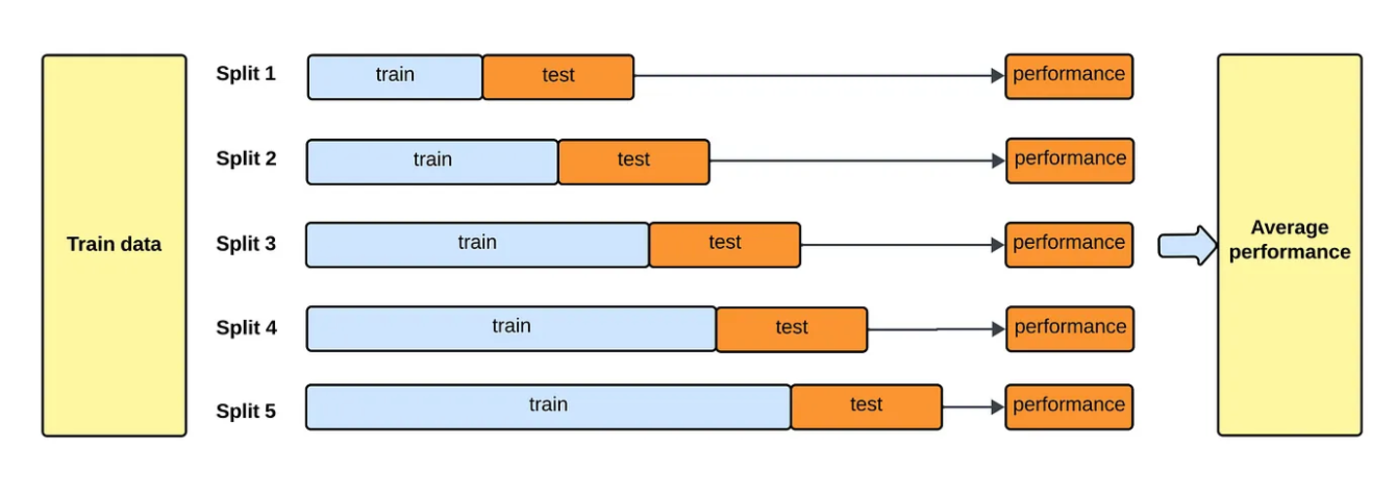
\includegraphics[width=400pt]{cross_validation_timeseries.pdf}
	\caption{An illustration of the cross-validation process for time series analysis.\label{figure:cross_validation}} ~\\
\end{figure}


$k$-fold cross-validation provides a more robust estimate of the model's performance compared to a single train-test split, as it evaluates the model on multiple subsets of the data. It also helps in detecting overfitting by assessing the model's generalization ability across different subsets of data\footnote{For documentation, the code used in the \texttt{KFold} function from the \texttt{scikit-learn} package, please refer to \href{https://scikit-learn.org/stable/modules/cross\_validation.html}{https://scikit-learn.org/stable/modules/cross\_validation.html}.}. \\

We also consider leave-one-out cross-validation (LOOCV), which is a special case of $k$-fold cross-validation. Here, $k$ is equal to the number of samples in the dataset. In LOOCV, the model is trained $k$ times, each time leaving out one sample for testing and training on the remaining samples. This process is repeated for each sample in the dataset, and the performance metrics are averaged across all iterations to obtain the final evaluation metric. \\

$k$-fold cross-validation strikes a balance between computational efficiency and robustness by dividing the dataset into smaller subsets, whereas LOOCV exhaustively trains the model on nearly all possible combinations of training and testing samples, making it computationally expensive for larger datasets. $k$-fold cross-validation provides a more efficient estimate of model performance and is more commonly used in practice. \\

\section{What is LARS Lasso Regression?}

LARS Lasso regression is a regularized linear regression technique that combines the Least Angle Regression (LARS) algorithm with the Lasso (Least Absolute Shrinkage and Selection Operator) regularization. It is useful when dealing with high-dimensional data or when feature selection is desired. \\

The main idea behind LARS Lasso is to efficiently solve the Lasso regression problem, which aims to minimize the sum of squared residuals while imposing an L1 penalty on the regression coefficients. The L1 penalty encourages sparsity in the coefficients, effectively shrinking some of them to exactly zero. This property makes Lasso regression well-suited for feature selection, as it automatically identifies and selects the most relevant features for the model. \\

The LARS algorithm is used to efficiently compute the Lasso solution path, which is the sequence of regression coefficients as the regularization parameter varies. It starts with all coefficients equal to zero and iteratively adds or removes variables based on their correlation with the residual. The algorithm proceeds in a stepwise manner, gradually increasing the magnitude of the coefficients until all variables are included in the model or a certain stopping criterion is met. \\

One of the key advantages of LARS Lasso is its computational efficiency. It can handle high-dimensional data with a large number of features relatively quickly compared to other regularization techniques. Additionally, the Lasso regularization helps to prevent overfitting by constraining the magnitude of the coefficients and promoting a simpler and more interpretable model. \\

When using LARS Lasso, the regularization parameter (often denoted as $\lambda$) controls the strength of the L1 penalty. A higher value of $\lambda$ leads to more regularization and sparser coefficients, while a lower value allows for more complex models. The optimal value of $\lambda$ is determined through techniques such as cross-validation, as described above. \\

\section{What is Desmoothing?}

\begin{figure}[!h]
	\centering
	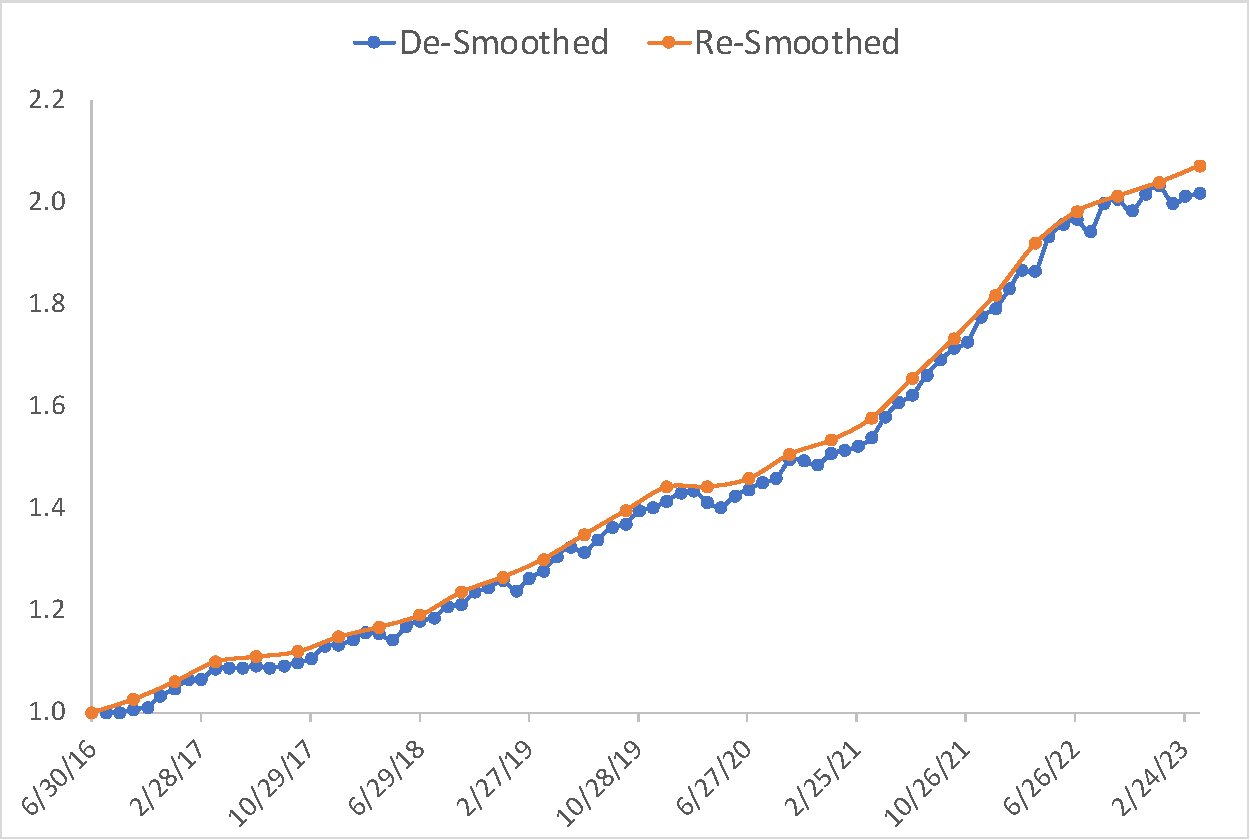
\includegraphics[width=400pt]{desmoothed.pdf}
	\parbox{425pt}{\caption{An example of a fund’s de-smoothed ($x$), and re-smoothed ($y$) returns as generated by GMAM 3. The reported re-smoothed returns are quarterly, and the de-smoothed returns are monthly. Shown here is the cumulative return of \$1 invested in each of the set of returns. }}
\end{figure}

It is well-known in the finance practitioner literature that returns from alternative investment such as PE, hedge funds, or real estate funds are highly serially correlated (see, for example, Getmansky, et al. (2004)\footnote{Getmansky, M., A. Lo, and I. Makarov. 2004. An Econometric Model of Serial Correlation and Illiquidity in Hedge Fund Returns. \textit{Journal of Financial Economics}, 74(3):529–609.}. In other words, past values correlate with present values. The serial correlation occurs because of the lack of liquidity in the fund itself or some of the assets held within it. For instance, these illiquid assets may not trade frequently, leading to subjective and otherwise noisy valuations.  The effect is such that when funds contain illiquid assets, their reported returns may seem steadier than their actual economic returns (returns that consider all available market information about those securities). The positive serial return correlation commonly leads to a downward bias in estimated return variance, or a  smoothing effect. \\

The effect extends to the reported returns of real estate funds(see, for example, Geltner (1993)\footnote{Geltner, D. 1993. Estimating Market Values from Appraised Values Without Assuming an Efficient Market. \textit{The Journal of Real Estate Research}, 8(3):324–345.}. Investors typically demand monthly or quarterly reporting. But valuations of many properties included in the funds are effectively updated only annually. Each quarter some properties have their valuations updated, and others do not. For some properties, the lack of a new valuation within a quarter might result in a carry-over of their last known value into the current quarter.  \\

Finally, Financial Accounting Standard 157, released by the FASB in 2006 during the run-up to the financial crisis, and now called Accounting Standards Code Topic 820, requires companies to mark their assets to market. The rule was a radical change from historic cost accounting and required general partners to periodically mark the assets to market. This may also result in a managerial bias towards smoothing asset values. \\

The latent returns $x_{i,t}$, henceforth just $x$ for simplicity of notation, generated above are not smoothed. They are the true economic returns. Since GMAM 3 attempts to mimic true reported returns, we must re-smooth the latent returns to reflect the reported returns so that investors can appropriately compare their investments in Alts with publicly available investments. In GMAM 3, this is done using a moving average (MA) process with smoothing parameters estimated using a Bayesian linear regression. Note that the MA is defined in an econometric sense, and not in a literal sense, although it may be interpreted as such. More specifically, the final returns presented to the user are re-smoothed using the following process:
\begin{equation}
\label{eq:y}
	y=\Phi x
\end{equation}

where $y$ are the reported returns; $\Phi$ is a matrix consisting of smoothing coefficients, $\phi$ and $\tilde{\phi}$ defined in more detail below); and $\mathbf{x}$ is a vector of $x$ values. When both $x$ and $y$ have the same reporting frequency:
\begin{equation}
\label{eq:phi}
	\Phi =
	\begin{bmatrix}
		\phi_{1} & \cdots & \phi_{P} & \tilde{\phi}_{P+1} & 0 & 0 & 0 & 0 & 0\\
		0 & \phi_{1} & \cdots & \phi_{P} & \tilde{\phi}_{P+1} & \cdots & \cdots & \cdots & 0\\
		\vdots & \ddots & \ddots & \ddots & \ddots & \ddots & \ddots & \ddots & \vdots\\
		0 & \cdots & \cdots & \cdots & \phi_{1} & \cdots & \phi_{P} & \tilde{\phi}_{P+1} & 0\\
		0 & \cdots & \cdots & \cdots & \cdots & \phi_{1} & \cdots & \phi_{P} & \tilde{\phi}_{P+1}
	\end{bmatrix} 
\end{equation}

$\phi$ is a vector of $P$ unrestricted coefficients, and $\tilde{\phi}$ is a vector of $P + \Delta t$ restricted and unrestricted coefficients. $P$ and $\Delta t$ represent terms that map the observation period of the reported, smoothed returns $y$ to the latent, de-smoothed returns, $x$. \\

The reported returns are $y_s$ s.t. $s \in 1:S$, and the latent returns are $x_t$ s.t. $t \in 1:T$. In equation \eqref{eq:phi} above, $S = T-P$, and the reported returns and de-smoothed returns have the same frequency. However, $S$ may not always equal $T$; for example, when the reported returns are quarterly, and the de-smoothed returns are monthly. To resolve this, the following formula maps $t$ to $s$:
\begin{equation}
	t(s) = P + (s \times \Delta t)
\end{equation}

For example, if the reported returns $y$ are quarterly, and the latent returns $x$ are monthly, $P=3$, and $\Delta t = 3$ (since each quarter consists of three months). And so, for the first quarter, $s = 1$, and $t = 6$. When $\Delta t > 1$, the values in $\tilde{\phi}_j$ must add up to $1$ for each month of the quarter (first, second, third). If not, months that fall earlier in the quarter will have a different long-run impact on NAV than months later in the quarter. For instance if we have a single quarter lag, the first month of the quarter plus the first month of the previous quarter must add to $1$. This implies that the sum total of values in $\tilde{\phi}_j$ is $3$ for quarterly data and $1$ for monthly data.\footnote{Note that the vector $\phi \in \tilde{\phi}$. For quarterly reported data, say $\phi = [a, b, c]^\prime$ where $a, b, c \in \mathbb{R}$. Then, $\tilde{\phi} = [a, b, c, 1-a, 1-b, 1-c]^\prime$ and the sum of all terms in $\tilde{\phi}$ is 3. For monthly reported data, say $\phi = [a, b, c, d, e]^\prime$ where $a, b, c, d,e \in \mathbb{R}$. Then $\tilde{\phi} = [a, b, c, d, e, 1-a-b-c-d-e]^\prime$ and the sum of all terms in $\tilde{\phi}$ here, is 1. This process is also described in more detail in the Appendix.}.  \\

In particular,
\begin{align}
	y_{s} 	&= \left(\tilde{\phi}_{1:\left(P+\Delta t\right)}\right)'x_{(t[s]-P-\Delta t+1):t[s]}+\varepsilon_{t}^{y}	\\
			&= \left(\tilde{\phi}_{\left(P+1\right):\left(P+\Delta t\right)}\right)'x_{\left(t[s]-\Delta t+1\right):t[s]}+\phi'x_{(t[s]-P):\left(t[s]-\Delta t\right)}+\varepsilon_{t}^{y}
\end{align}

The complete posterior distribution of $y$ is given by:
\begin{equation}
\label{eq:y_dist}
	p \left( y \mid rest \right) \sim MN \left( \Phi x,\frac{1}{\tau_{y}}I\right))
\end{equation}

where $\tau_y$ is a global precision parameter estimated for independent measurement variance. The precision parameter has Gamma-distributed prior: $p( \tau_y ) \sim Gamma \left( \alpha_{y_0}, \zeta_{y_0} \right)$ with given shape hyperparameter, $\alpha_{y_0}$, and given inverse scale hyperparameter, $\zeta_{y_0}$;  $\tau_\phi$ is a global precision multiplier parameter, distributed as $p( \tau_\phi ) \sim Gamma \left(\alpha_{\phi_0}, \zeta_{\phi_0} \right)$ with given shape and inverse scale hyperparameters; $M_0$ is a $P \times P$ matrix consisting of precision hyperparameters for $\phi_0$; and $\phi_0$ is a hyperparameter (i.e., fed into the model). \\

The economic assumption behind the smoothing process is simple: that the observed fund returns ($y$) are a weighted average of the fund’s economic returns $x$ over the most recent ($P + \Delta t$) periods, inclusive of the current period. The econometric implications of this are that under the given assumption, the observed fund returns follow a MA process of order $P + \Delta t$. \\

This restriction is similar to Getmansky, et al. (2004) where the observed return ($R_t^0$) for some period $t$, is a weighted average of the 	``true'' returns ($R_t^C$) over the most recent $k+1$ periods: $R_t^0 = \theta_0 R_t^C + \cdots + \theta_k R_(t-k)^C$, with $\sum_{i=0}^k \theta_i  = 1$ to ensure that all information is eventually incorporated into observed returns, and $\theta_i \in [0,1]$ for $i = 1, \ldots, k$. In our case the observed returns are the reported returns, $y$, the ``true'' returns are the latent returns generated using the factors, $x$, and the $\theta_i$ terms from Getmansky, et al. (2004) are denoted as $\phi_i$ in our estimation process. They are generated using a multivariate normal distribution in the hierarchical Bayesian model, as follows:

\begin{equation}
\label{eq:phi_dist}
	p\left(\phi|rest\right) \sim MN\left(\phi_{0},\frac{1}{\tau_{y}\tau_{\phi}}M_{0}^{-1}\right)
\end{equation}

where $\tau_y$ is as defined above; $\tau_\phi$ is a global precision multiplier parameter, distributed as $p( \tau_\phi ) \sim Gamma \left(\alpha_{\phi_0}, \zeta_{\phi_0} \right)$ with given shape and inverse scale hyperparameters; $M_0$ is a $P \times P$ matrix consisting of precision hyperparameters for $\phi_0$; and $\phi_0$ is a hyperparameter (i.e., fed into the model). 



%\newpage
%
%\section*{GMAM 3 Redux}
%
%The asset return at time $t$, denoted by $y_t$, is modeled as:
%\begin{equation}
%    y_t = F_t^\top\beta_t + \epsilon_t
%\end{equation}
%where $F_t$ is a $K \times 1$ vector of observed factor returns, $\beta_t$ is a $K \times 1$ vector of time-varying factor exposures, and $\epsilon_t$ is the idiosyncratic error term.
%
%\subsection*{Factor Exposure Dynamics}
%
%The factor exposures $\beta_t$ follow a sparse vector autoregressive process with stochastic volatility:
%\begin{align}
%    x_t &= F_t^\top\beta_t + \text{cash}_t \\
%    x_t &= \phi_1 x_{t-1} + \ldots + \phi_P x_{t-P} + \eta_t \\
%    \eta_{t,k} &\sim \begin{cases}
%        N(0, \tau_\beta^{-1}), & \text{if } \gamma_{t,k} = 1 \\
%        0, & \text{if } \gamma_{t,k} = 0
%    \end{cases} \\
%    \gamma_{t,k} &\sim \text{Bernoulli}(\omega_t) \\
%    \omega_t &\sim \text{Beta}(\kappa_0, \delta_0)
%\end{align}
%where $\phi_1, \ldots, \phi_P$ are $K \times K$ autoregressive coefficient matrices, $\eta_t$ is a sparse innovation term with stochastic volatility controlled by $\tau_\beta$, and $\gamma_{t,k}$ is a binary random variable determining the sparsity of the $k$-th element of $\beta_t$.
%
%\subsection*{Idiosyncratic Error Distribution}
%
%The idiosyncratic error term $\epsilon_t$ follows a Student's t-distribution with time-varying degrees of freedom $\nu_t$ and scale $\tau_y^{-1/2}$:
%\begin{align}
%    \epsilon_t &\sim t_{\nu_t}(0, \tau_y^{-1/2}) \\
%    \nu_t &\sim \text{TruncatedGamma}(\alpha_{\nu_0}, \zeta_{\nu_0}) \\
%    \tau_y &\sim \text{Gamma}(\alpha_{y_0}, \zeta_{y_0})
%\end{align}
%where $\nu_t$ governs the heaviness of the tails of the Student's t-distribution, and $\tau_y$ is the stochastic volatility parameter for the idiosyncratic errors.
%
%\subsection*{Prior Distributions}
%
%The model incorporates the following prior distributions:
%\begin{align}
%    \phi_i &\sim N(m_0, \tau_\phi^{-1} I), & \tau_\phi &\sim \text{Gamma}(\alpha_{\phi_0}, \zeta_{\phi_0}) \\
%    \beta_0 &\sim N(\beta_{\delta_0} / d, \tau_\beta^{-1} A_0), & \tau_\beta &\sim \text{Gamma}(\alpha_{\beta_0}, \zeta_{\beta_0}) \\
%    A_0 &= \text{diag}(a_0 d^2), & d &= \sqrt{\gamma + (1-\gamma)/v^2}
%\end{align}
%where $\kappa_0, \delta_0, v, \alpha_{\nu_0}, \zeta_{\nu_0}, \alpha_{y_0}, \zeta_{y_0}, \alpha_{\phi_0}, \zeta_{\phi_0}, \alpha_{\beta_0}, \zeta_{\beta_0}, a_0, m_0$ are hyperparameters.
%
%\subsection*{Auxiliary Variables}
%
%The model involves the following auxiliary variables:
%\begin{align}
%    \psi_t &= \text{Gamma}(\nu_t/2, \nu_t/(2\tau_x\tau_y(x_t - \mu_x)^2)) \\
%    \mu_x &= E[x_t | \beta_t] \\
%    \tau_x &\sim \text{Gamma}(\alpha_{x_0}, \zeta_{x_0})
%\end{align}
%where $\mu_x$ is the conditional expectation of $x_t$ given $\beta_t$, and $\tau_x$ is the stochastic volatility parameter for $x_t$.





\newpage

\bibliographystyle{ledgerbib}
\bibliography{FactorReturnsProjection}
\nocite{*}


%AUTHOR: comment out, this is used to make sure the Creative Commons License
%image fits on page

\newpage

%define the following sections to have the Appendix Style

%\appendix
%\setcounter{section}{0}
%\section{Data and Descriptions}





%\newpage
%here up^^


\thispagestyle{pagelast}





%\theendnotes

\end{document}
